%-------------------------------
% 4YP REPORT
%-------------------------------

% JAMES ROUTLEY

% COMPILE WITH XeLaTeX

%-------------------------------
% Preamble
%-------------------------------
\documentclass[11pt, a4paper]{report}
\linespread{1.669} % similar to double line spacing in word
\usepackage[margin=20mm]{geometry}
\usepackage{fontspec, amsmath, url}
\usepackage[hang,small]{caption} % make captions look better
\usepackage{url, hyperref}
\usepackage[backend=bibtex, sorting=none]{biblatex}
\bibliography{4yp}
\setmainfont{Arial}
\setlength{\parindent}{0in}
\setlength{\parskip}{0.5cm}
\newcommand{\HRule}{\rule{\linewidth}{0.5mm}}
\newcommand{\vect}[1]{\boldsymbol{#1}}



%-------------------------------
% Document
%-------------------------------
\begin{document}




%-------------------------------
% Title
%-------------------------------
\begin{titlepage}
\begin{center}

% Upper part of the page. The '~' is needed because \\
% only works if a paragraph has started.
% \includegraphics[width=0.15\textwidth]{./logo}~\\[1cm]

\includegraphics[width=0.16\textwidth]{img/OxfLogo.png}~\\[1.5cm]

\textsc{\LARGE University of Oxford}\\[1.5cm]
\textsc{\Large Fourth year project}\\[0.5cm]

% Title
\HRule \\[0.4cm]
{ \huge \bfseries A Flower Classification Application \\[0.4cm] }

\HRule \\[1.5cm]

% Author and supervisor
\noindent
\begin{minipage}[t]{0.4\textwidth}
\begin{flushleft} \large
\emph{Author:}\\
James \textsc{Routley} \\
Trinity College
\end{flushleft}
\end{minipage}%
\begin{minipage}[t]{0.4\textwidth}
\begin{flushright} \large
\emph{Supervisors:} \\
Professor~Andrew \textsc{Zisserman} \\
Yuning \textsc{Chai}
\end{flushright}
\end{minipage}

\vfill

% Bottom of the page
{\large May 2015}

\end{center}
\end{titlepage}









%-------------------------------
% Contents
%-------------------------------
\setlength{\parskip}{0.0cm}
\tableofcontents
\setlength{\parskip}{0.4cm}


%-------------------------------
% Introduction
%-------------------------------
\chapter{Introduction}

\section{Definition of the problem} 

\section{Why problem is worth solving, challenges which occur during this type of classification}

Considerably higher accuracy can be achieved using computer vision techniques when compared to human classification. 

\section{Description of data}

This project makes use of the Oxford 17 category flower dataset and the Oxford 102 category flower dataset. 

'Both contain sets of images of flowers which commonly occur in the United Kingdom. The images have large scale pose and light variations. In addition, there are categories that have large variations within the category and several very similar categories.' - ?

The 102 dataset are split into training, validation and test sets.

The more manageable 17 dataset was used at first to get an overview of the classification process.

Once an initial classification pipeline was developed, the more comprehensive 102 dataset was used. 

\section{Achievements}






%-------------------------------
% Literature Review
%-------------------------------
\chapter{Literature review}

(3-5 pages long. Gives reader knowledge of what people have done before on this topic.) 

This project builds on work done by the Oxford University Visual Geometry Group on the flower classification problem. (check which papers to cite)

Chai et al.~\cite{Chai11} (check bibtex - is inProceedings correct?), on 

\section{Automatic visual classification apps}

Similar apps:
Leafsnap - iPhone application which uses computer vision techiniques to identify trees based on leaf images. Covers the 185 tree species in Northeastern US. Uses image segmentation (\url{http://neerajkumar.org/base/papers/nk_eccv2012_leafsnap.pdf}). Uses image segmentation and leaf shape as the principle classification metric. 

Dog classification:
\url{http://www.umiacs.umd.edu/~kanazawa/papers/eccv2012_dog_final.pdf}

Google googles (very broad - too broad?):
\url{https://play.google.com/store/apps/details?id=com.google.android.apps.unveil&hl=en_GB}


 (there are for dogs, leaves) - look up these papers and compare them.

\section{Flower classification apps}
Whilst these do exist, most either provide a database of plant knowledge which the user then manually searches through:

(\url{https://play.google.com/store/apps/details?id=org.pottssoftware.agps21}, 
\url{https://play.google.com/store/apps/details?id=com.luontoportti}, 
\url{https://itunes.apple.com/us/app/ipflanzen/id416983587?mt=8}), 

or use a large network of users to crowdsource a classification. 

(\url{https://play.google.com/store/apps/details?id=cz.thran.flowerchecker}, \url{https://play.google.com/store/apps/details?id=org.plantnet&hl=en})


\section{Flower Classification}

Look over previous papers on flower classification (\url{http://www.robots.ox.ac.uk/~vgg/research/flowers_demo/index.html}	)

\section{Convolutional Neural Networks}

CNNs, where they came from, who invented them, imagenet challenge (\url{http://www.image-net.org/}), image depicting CNN architecture. 


Description of LibLinear?












%-------------------------------
% Classification
%-------------------------------
\chapter{Classification}

\section{Overview of classification pipeline}

\begin{figure}[hbt]
	\centering
  \includegraphics[totalheight=3cm]{img/08.png}
  \caption{(a): Convolutional neural network inspired feature extraction. An image is supplied to the convolutional neural network which generates its feature vector $\vect{x}$, which describes the content of the photograph. (b): Support vector machine image classification. The vector is compared to the previously found weight vectors $\vect{W}$, producting a vector of prediction values, $\vect{p}$. (c) The index $i$ of the maximum value in $\vect{p}$ is found, which gives the classification result $i$.}
  \label{img:08}
\end{figure}


\section{Convolutional neural network (CNN) inspired feature extraction}

The pipeline makes use of the first six layers of the fast convolutional neural network CNN-F introduced in “Chatfield et al.~\cite{Chatfield14}. This algorithm takes a photo as its input and produces a vector which describes the features of the photo. The photo is cropped to 224x224 pixels and normalised before use and the outputted feature vector is also normalised.

The CNN is trained on the ImageNet Large Scale Visual Recognition Challenge 2012 (ILSVRC2012) dataset~\cite{CNN:Imagenet}. Details of the training can be found in ~\cite{Chatfield14}. The feature extraction process itself is treated as a black box in this project. 

 


\section{Support vector machine (SVM) image classification}

\subsection{How SVMs are used in the classification pipeline}

The classification pipieline uses the open source support vector machine (SVM) library LibLinear~\cite{SVM:LibLinear} for quick, large scale classification. One-vs-the-rest classification is used. $n$ SVM models are trained for $N$ flower categories, producing $N$ weight vectors, $\vect{w_{1}}, \vect{w_{2}}, ..., \vect{w_{N}}$. These weight vectors are stacked into a weight matrix $\vect{W}$: 
$$
\vect{W} = 
\begin{pmatrix}
\vect{w_{1}}\\  
\vect{w_{2}}\\ 
\vdots \\ 
\vect{w_{n}}
\end{pmatrix}
$$



During classification, the scalar product of the unseen flower's feature vector, $\vect{x}$ and each of the weight vectors is calculated, to produce a vector of prediction values, $p_{1}, p_{2} ... p_{n}$:
$$
\vect{W} \cdot \vect{x} =
\begin{pmatrix}
p_{1}\\  
p_{2}\\ 
\vdots \\ 
p_{n}
\end{pmatrix}
$$

The value of $p_{i}$ indicates how closely the unseen flower's features matched those of category $i$. The higher the product, the more closely they match. The unseen flower's category is therefore predicted to be that which produced the greatest prediction value. 



\subsection{Training and testing SVMs}

Before use, the SVM model $\vect{W}$ must be trained. They are trained using a set of images which are known to be of certain categories. These models are then tested, using a set of images also known to be of certain categories, to check they are sufficiently accurate. 

The C parameter of the SVM must be adjusted. The C Parameter allows for a solution with a larger margin, in return for the violation of some constraints. To find the optimal C Parameter, SVM models are trained using the training set images  before testing against the validation set images. The change in classification accuracy is recorded as the C Parameter is changed. 



\subsubsection{Training} 

SVM models are trained using LibLinear's training function. To train a model to recognise a flower category $i$, all photos in the training and validation sets are passed to the training function, with the photos of category $i$ labeled as in the category, and all other flowers labeled as not in the category. The flowers are labeled as in or not in the category by passing a 1 or -1 respectively to the training function, alongside that flower's feature vector.

The training function produces a weight vector of order 4096, which describes the characteristics of the flowers in that category. %The similarity between a new flower and those in the category can be found by comparing the new flower's feature vector and the category's weight vector.

\subsubsection{Testing}

Testing allows the quality of each SVM model to be checked. Testing uses the test subset of the flower datasets. Each flower in the test set is run against each of the SVM models generated during training. The dot product of the  flower's feature vector and each of the model's weight vectors is found. The greater the result of the dot product, the greater the correlation between the tested flower and that category. Thus the category which produces the greatest dot product result is predicted to be the category of the flower.

By comparing the actual categories of the flowers in the test set to the predicted categories, an overall percentage accuracy can be calculated.


\section{Experiments}
%TODO aim to make this section 7 pages

\subsection{SVM accuracy}

\subsubsection{How we define accuracy}

Accuracy is defined as the percentage number of correct classifications, where under correct classification, the category of the model which most closely identifies with the flower is indeed the category of that flower:
$$
Accuracy = \frac{Number\ of\ correctly\ classified\ flowers}{Total\ number\ of\ flowers}
\times 100
$$

Accuracy is found by classifying all images in the test sets, and checking the classified categories against the actual categories. 

\subsubsection{Rank accuracy}

Rank accuracy measures the percentage accuracy of the correct category being in the top $K$ classified categories. As a user will be receiving results on their phone, a selection of likely flower categories can presented to that user, who can make the final decision. How rank accuracy changes as we consider more ranks therefore can give us an indication as to how many results to present the user. The more results are presented, the more likely the correct classification will be included, but the more cluttered the presentation is.
$$
Rank\ accuracy = \frac{Number\ of\ correctly\ classified\ flowers\ considering\ the\ top\ K\ results}{Total\ number\ of\ flowers}
\times 100
$$



\subsection{Improving SVM accuracy}

\subsubsection{Mirroring and sampling training set images}

\begin{figure}[hbt]
	\centering
  \includegraphics[totalheight=4cm]{img/09.png}
  \caption{An example flower shown with its vertical mirror}
  \label{img:09}
\end{figure}

\begin{figure}[hbt]
	\centering
  \includegraphics[totalheight=8cm]{img/10.png}
  \caption{An example flower shown with the images sampled from it}
  \label{img:10}
\end{figure}

Taking mirrors and samples of the images in the test set (Figures~\ref{img:09} and~\ref{img:10}) allows the test set to be expanded. The objective of this is to get the most out of the training set images. Both techniques generate new images from which new feature vectors can be calculated. These can be used to improve the quality of the SVM model. 

Only the vertical mirror can be used, as shown in Figure~\ref{img:09}, as flowers only exhibit vertical symmetry. 


\subsubsection{Mirroring and sampling test images}

For the same reasons as laid out above, mirroring and sampling the test image can improve classification accuracy.

For each image, several image vectors $\vect{x_{i}}$ are now being produced. Each one of these is run against the weight matrix to produce several vectors of prediction values $\vect{p_{i}}$. To classify the flower, these vectors of prediction values must be combined. This can be done by finding the mean of each corresponding value, or by taking the maximum of each corresponding value:
$$
\begin{aligned}
	\vect{x} &= \sum_{n = 0}^{n} \vect{x}_{i} \\
	& or \\
	&= max(\vect{x}_i)
\end{aligned}
$$

%TODO complete analysis when completed
(I've implemented this, and see a 1-2\% increase in accuracy - need to discuss how to present data in supervision)


\subsection{Results}

\begin{table}[h]
\centering 
\renewcommand{\arraystretch}{1.3}
\begin{tabular}{l|cc}
  & {\bf 17 flower dataset} & {\bf 102 flower dataset} \\
  \hline
  Baseline & 89.8 $\pm$ 0.68\% & 85.1 $\pm$ 0.59\% \\
  Mirroring & 89.4 $\pm$ 0.82\% & 85.5 $\pm$ 0.68\% \\
  Sampling & 89.7 $\pm$ 0.75\% & 84.3 $\pm$ 0.39\% \\
  Mirroring and Sampling & 90.3 $\pm$ 0.73\% & 85.2 $\pm$ 0.24\% 
\end{tabular}
\renewcommand{\arraystretch}{1}
\caption{Mean classification accuracy and standard devaition for the Oxford 17 and 102 flower datasets while using the standard, mirrored and subsampled training image sets}
\label{table:accuracy}
\end{table}

If the images in the test set happen to closely match those in the training set, the classification accuracy would be higher than if the opposite were true. To account for these idiosyncrasies, the script which calculates classification accuracy is run five times. Each time it uses 20 randomly selected images as the training set and the rest of the images as the test set. The mean accuracy and the standard deviation of the results are found. 20 images are used as this is the number of images used in the training set defined in the dataset. 

\subsection{Analysis of results}
%Standard Deviation low, indicating good something
%
%Mirror and Sampling have little effect on accuracy - these effects could already be looked at by the CNN
%
%% (100) finish once results in
%Confusion Matrices allow deeper analysis of results. Certain categories perform badly. This explain why (similar looking flowers? - give photos)
%(add confusion matrix analysis)
%
%%TODO talk about the visualisation website?

The standard deviations of the results are low, indicating that the accuracy figures are reliable, and the accuracy rates are high. These accuracies are obtained using models trained on subset of the total images available. The final models used for the application are trained on all the images, and should have higher accuracy rates.

The following sections make use of tools for further analysis of results. 

\subsubsection{Confusion matrices}

%TODO rewrite
Confusion matrices give a more detailed view of the classification. It presents the classification results as a series of rows. Each row represents a category being classified and the numbers in that row show what percentage of the test images were classified as that category. 

For example, for the images tested from category 1 of the 17 flower dataset. 53\% were correctly classified as category 1, 3\% were classified as category 5, 10\% as 8 and 35\% as 14.

(add further analysis - talk about how some flowers look like others (e.g. 14 in 17dataset is particularly strong). Also category 10 in the 17 database has 100\% accuracy without any other species being misclassified to it. Probably distinctive. Add images of the flowers in question.)


\begin{figure}[hbt]
	\centering
  \includegraphics[totalheight=15cm]{img/15.png}
  \caption{Confusion matrix for the 17 flower dataset, obtained using mirroring and sampling}
  \label{img:15}
\end{figure}

%TODO figure
\begin{figure}[hbt]
	\centering
  \includegraphics[totalheight=15cm]{img/16.png}
  \caption{Confusion matrix for the 102 flower dataset, obtained using mirroring and sampling}
  \label{img:16}
\end{figure}

\subsubsection{Rank accuracy}

The rank accuracy graph shows that classification accuracy quickly increases as more ranks are considered (Figure~\ref{table:rank}). This backs up the presentation of several choices to the user, who makes the final classification choice. 


%TODO add more
(decide on number of ranks to show the user - the more there are the higher the accuracy rate, but the more complex the app experience is. I'm thinking 6?)  





\begin{table}[h]
\centering 
\renewcommand{\arraystretch}{1.3}
\begin{tabular}{c|cc}
  {\bf Number of}\\ {\bf ranks considered} & {\bf 17 flower dataset} & {\bf 102 flower dataset} \\
  \hline
  1 & 90.3\% & 85.2\% \\
  4 & 98.6\% & 94.6\% \\
  6 & 99.3\% & 95.7\% \\
  8 & 99.6\% & 96.8\% \\
  10 & 99.8\% & 97.5\% 
\end{tabular}
\renewcommand{\arraystretch}{1}
\caption{Classification accuracies obtained when considering different numbers of ranks for the 17 and 102 flower datasets, using both mirroring and sampling}
\label{table:rank}
\end{table}

\begin{figure}[hbt]
	\centering
  \includegraphics[totalheight=8cm]{img/19.png}
  \caption{Confusion matrix for the 17 flower dataset, obtained using mirroring and sampling}
  \label{img:19}
\end{figure}

\begin{figure}[hbt]
	\centering
  \includegraphics[totalheight=8cm]{img/21.png}
  \caption{Rank accuracy for 102 flower dataset, using both mirroring and sampling}
  \label{img:21}
\end{figure}



%-------------------------------
% Client and Server Architecture
%-------------------------------
\chapter{Client and server architecture}
% This chapter describes the code behind the client and server. 

\section{Overview of client and server architecture}

\begin{figure}[h]
	\centering
  \includegraphics[totalheight=3cm]{img/11.png}
  \caption{The classification system is made up of two parts, a client and a server. The client is an application running on a user's Android phone. The application allows the user to upload a photo to the server. The server performs the classification, before returning the results to the application, where they are displayed.}
  \label{img:11}
\end{figure}


\section{Client architecture} 

\begin{figure}[h]
	\centering
  \includegraphics[totalheight=9cm]{img/12.png}
  \caption{Diagram showing the information flow between different sections of the client}
  \label{img:12}
\end{figure}

The client is an Android application which is made up of three activities~\cite{AndroidDev:Activity}. Each activity is an object which allows the user to perform a specific task, and has a screen which which the user can interact with it. The functions of the activities are shown in Figure~\ref{img:12}. Screenshots of the activities are shown in Figure~\ref{img:03} 



\subsection{Taking the photo}

After the application is launched, the Main Activity of the application (Figure~\ref{img:12} (a)) presents the user with two buttons, which allow the user to take a photo, or upload a photo previously taken from a gallery. Both of these buttons trigger intent calls. Intents are objects native to the Android system, which allow an application to request an action from another app component. The intent call starts the built-in camera or the gallery application, and allows the user to take or pick a photo without having to write that code into the application. 

Once a photo is taken or chosen, the second activity of the application (Figure~\ref{img:12} (c)) is called, and the filename of the photo is passed to it. 

%\begin{figure}[hbt]
%	\centering
%  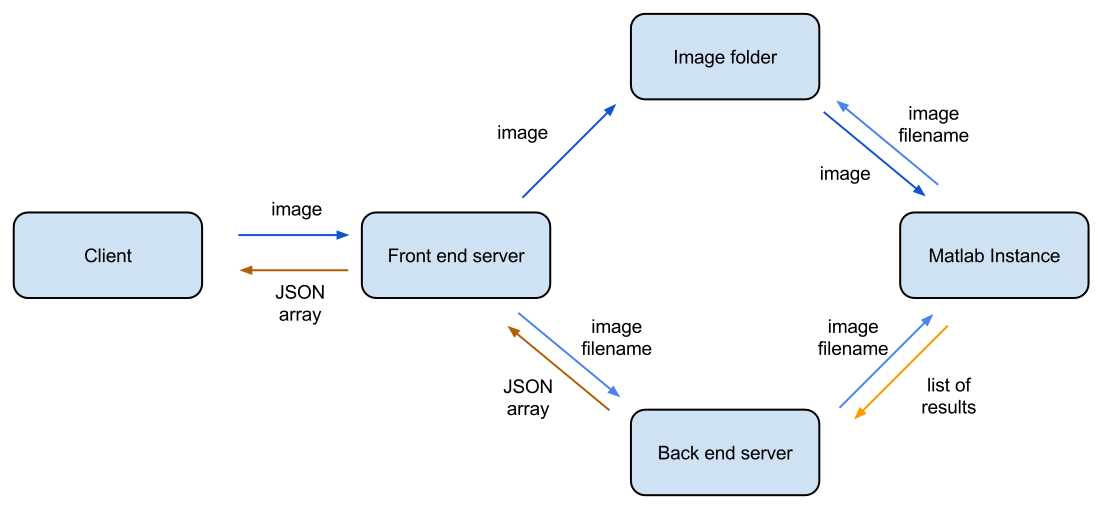
\includegraphics[totalheight=6cm]{img/01.png}
%  \caption{Illustration of how an implicit intent is delivered through the system to start another activity: [1] Activity A creates an Intent with an action description and passes it to startActivity(). [2] The Android System searches all apps for an intent filter that matches the intent. When a match is found, [3] the system starts the matching activity (Activity B) by invoking its onCreate() method and passing it the Intent.}
%  \label{img:01}
%\end{figure}

\subsection{Uploading the photo}

As the Results Activity (Figure~\ref{img:12} (b)) is called, a HTTP connection is opened, connecting to the URL of the server. A HTTP POST request is started, and the photo is uploaded to the server. The filename is appended to the POST request header as the value in a key-value pair. The key is predetermined and is known by the client and server and is used by the server to extract the image from the body of the request. 

The object which contains the code to upload the image extends a native Android object called an AsyncTask~\cite{AndroidDev:AsyncTask}. The AsyncTask starts a new thread, and runs the upload code on it. This is done because the photo upload can take several seconds. If this were to take place on the user interface thread, user interface features such as scrolling and use of the navigation buttons could not take place until the uploading had done. This makes the application seem like it has frozen and is bad user experience design.

\subsection{Receiving results}

Once the photo has been uploaded to the server, and the classification has been carried out, the server responds with a JSON array containing the classification results and information about those flowers. 

The array consists of a number of flower objects, each of which contains the flower name, species, the URL of an example image, a snippet of information about the flower from Wikipedia and a links to that flower's Wikipedia page and google search.

The results are placed in a list, shown in Figure~\ref{img:03} (b), and the images are downloaded from their URLs using an image downloading and caching library named Picasso~\cite{AndroidDev:Picasso}. Picasso allows for the downloading, display and cacheing of an image with a single line of code. If an the user scrolls down the list and an image scrolled off the screen, it is destroyed in order to save memory space. If the user scrolls up again, the cacheing implemented by Picasso allows that same image to be loaded from memory, rather than be downloaded again. This improves performance as loading from memory is essentially instantaneous while downloading the image can take a few seconds.

If an image in the list is clicked, a detailed view of that flower is shown (Figure~\ref{img:03} (c)). This shows the user extra information about the flower, and presents them with buttons which allow them to Google search the flower or go to the flower's Wikipedia page. 



\section{Server architecture}


The server side consists of two servers. The first (front end) receives the image from the client, saves it to a folder and passes the filename to the second (back end) server. The second server calls a Matlab instance, and runs the Matlab classification script on the image. It constructs a JSON array of results and passes it to the first server which returns the results to the client. 

This two-server architecture improves security as file input and output is kept separate the classification logic.

\begin{figure}[hbt]
	\centering
  \includegraphics[totalheight=8cm]{img/07.png}
  \caption{Diagram showing information flow between the different sections of the server side}
  \label{svg:01}
\end{figure}

\subsection{Flask server}

The front end server runs the Flask server framework~\cite{Server:Flask}. The server sets up a URL and checks it for incoming POST requests. When a POST request is detected, it checks the request header, using a predetermined key, for the filename. It then uses the filename to download the image and save it to the image folder. 

Error catching is implemented as the incoming POST requests cannot be assumed to necessarily be benevolent. The filetype is checked and only image files are downloaded. Flask's \verb|secure_filename| function is used to generate filenames for the images before they are saved. The secure filename function stops filenames which could negatively affect computer behaviour, and prevents name clashes.

\subsection{Connection between servers}

\subsection{Backend server}

The backend server acts as a python wrapper around the Matlab classification code. It uses the python to Matlab bridge Mlwrap~\cite{Server:Mlwrap}, which allows Matlab functions as if they were python functions. 


Upon starting, the server opens an instance of Matlab, loads the convolutional neural network and the weight matrix $\vect{W}$. Each of these actions take several seconds but only need to be done once. By completing them upon start, they don't need to be run when a classification request is received, speeding up the classification time. 

It receives the filename from the front end server, and passes the filename and CNN to the Matlab classification function. This Matlab function returns a list of the category numbers of the eight top classification results. 

The backend server then constructs the JSON Array. Lists of flower names, species, image URL, Wikipedia text and Wikipedia and Google search URLs are stored. They are ordered by flower category such that the information for flower $i$ is stored at the $i^{th}$ for of the files. As the flower categories are numbered starting at $1$, the lists are indexed starting at $1$. The server uses the flower category numbers from the Matlab script to look up the appropriate information. This JSON array is passed back to the front end server which passes it to the client. 




%-------------------------------
% Application design
%-------------------------------
\chapter{Application design}
%"...describing the design of the app, showing screen shots of the interface as it goes through an example, plus a gallery of results."



\section{User interface design}

\begin{figure}[h]
\centering
\begin{minipage}[b]{0.2\linewidth}
	\centering
	\includegraphics[totalheight=6cm]{img/03.png}
	(a)
\end{minipage}
\begin{minipage}[b]{0.2\linewidth}
	\centering
	\includegraphics[totalheight=6cm]{img/05.png}
	(b)
\end{minipage}
\begin{minipage}[b]{0.2\linewidth}
	\centering
	\includegraphics[totalheight=6cm]{img/06.png}
	(c)
\end{minipage}
\caption{Screenshots of the screens seen by user. (a): The Main Activity allows the user to choose whether to take or upload a photo. (b): The Results Activity displays the classification results. (c): Detail Activity. If one of the images in (b) is clicked, a detail view of that flower is shown.}
\label{img:03}
\end{figure}

The user interface has been optimised by following Android's design guidelines~\cite{AndroidDev:Design}. This results in an Application which looks and behaves like applications the user has seen before, making it familiar and intuitive to use. 

\subsection{Material theme}

The application implements Android's recently released Material theme~\cite{AndroidDev:Material}. While the full Material theme can only run on devices running the latest version of Android, version 5.0 (API level 21), the look of the theme can be replicated on older devices by using Android's \verb|AppCompat| theme. 

\subsection{List and detail views}

The results of the classification are presented in a list (Figure~\ref{img:03} (b)), showing an image of the flower and the flower's common name. Above the list the photo the user has taken is shown, allowing for easy comparison. The images are cropped such that they are large enough to show the flower without taking up too much screen space. Each item on the list is clickable, and clicking reveals a page which details more information about that flower (Figure~\ref{img:03} (c)). This is a common way of presenting data and will be familiar to most users.


\subsection{Button and icon design}

\begin{figure}[hbt]
	\centering
  \includegraphics[totalheight=3cm]{img/13.png}
  \caption{The unpressed and pressed versions of the Take Photo and Upload Photo buttons}
  \label{img:13}
\end{figure}

The take photo and upload photo buttons are custom designed (Figure~\ref{img:13}), and use icons rather than words for simplicity. The icons used are adapted from the official Android icon pack~\cite{AndroidDev:Icons}, and will be familiar to Android users. The buttons use flat colour, keeping with the Material theme~\cite{AndroidDev:Material}. Both pressed and unpressed icons have been made, and the change in colour gives visual feedback to the user that the button has been pressed. 

(insert icon design when done)


\section{User experience design}

User experience has been optimised by focusing on making the classification as fast as possible and the application as simple to use as possible. 

\subsection{Simplification}

By keeping the application simple, it is easier to use. The application presents the user with a single choice; whether to take a photo or to upload a photo which has been previously taken. Uploading and downloading happens automatically, and no menu options are provided except the ability to share the result of a classification. 

\subsection{Flower images}

\begin{figure}[hbt]
	\centering
  \includegraphics[totalheight=8cm]{img/14.png}
  \caption{A selection of the hand-picked flower images shown to the user}
  \label{img:14}
\end{figure}

When the results are returned to the client, the images which are downloaded have been hand-picked for their quality. They have been chosen with the criteria of clearly display the flower in question, minimising any confusing background, and beauty. The images are cropped to the dimensions they will be displayed at, minimising the amount of data which needs to be transferred and speeding up the downloading time. 

%TODO maybe write something about finding most similar image

%\subsection{View hierarchy}

%TODO cite google's thing about useful back button if it can be found. 

\subsection{No good classification option}

It would appear unpolished if the application gave normal classification results for an image which is not a flower. If, after classification, the image does not closely match any of the categories ($p_{i} < -x \forall i = 1 ... n$), the user is notified, but the classification results are still provided.  

(TODO: run tests to find suitable x)


\chapter{Conclusions and future work}
Mirror of intro. Intro discusses challenges, conclusions describe how challenges were minimised. Were goals achieved

\section{Conclusions}

\section{Porting algorithm to Android}

%-------------------------------
% Bibliography
%-------------------------------
\printbibliography

\end{document}
